\documentclass{article}
\usepackage[a4paper, margin=1in]{geometry}
\usepackage{datetime}
\usepackage{wrapfig}
\usepackage[pdftex]{graphicx} \pdfcompresslevel=9
\newdate{date}{23}{02}{2024}
\date{Deadline : \displaydate{date}}

\title{TELECOM Graphisme par ordinateur: Projet Personnel}
\author{camille.schreck@inria.fr}

\begin{document}

\maketitle

Le rendu se fera par mail (camille.schreck@inria.fr). Le sujet du mail devra contenir [PROJET\_TNCY]. Le projet devra \^etre archiv\'e dans un fichier appel\'e \emph{projet\_nom\_prenom.zip} (ou .tar, .rar) contenant un dossier \emph{projet\_nom\_prenom} avec votre code, rapport et image.\newline
\newline
Le projet consiste \`a cr\'eer une sc\`ene dans Shadertoy.
Le sujet est libre mais le projet devra comporter:
\begin{enumerate}
\item au moins mouvement qui ne soit pas une rotation
\item plusieurs sources de lumi\`ere
\item un morceau de plan carr\'e non align\'e avec les axes sur lequel il y a une texture
\item un cylindre ouvert
\item un objet composé de plusieurs simples formes géometriques qui se d\'eplace (par exemple un cube compos\'e de six morceaux de plan, un personnage compos\'e de cylindres et sph\`eres...)
\item un effet diff\'erent de ce qu'on a fait en cours (miroir, objets semi-transparents, mat\'eriau sp\'eculaire, toon-shading...)
\item un c\^one.
\end{enumerate}
\vspace{1cm}
Le rendu devra comporter:
\begin{enumerate}
\item le code dans un (ou plusieurs si n\'ecessaire) fichier texte.
\item un rapport contenant
  \begin{itemize}
  \item un lien vers votre shader sur shadertoy
  \item une description de la sc\'ene et de ce que vous avez fait pour chacun des points ci-dessus (o\`u dans la sc\`ene, quelles formes, quels mouvements...)
  \item une explication de comment marche le code r\'ealis\'e pour le point 6
  \item les difficultés que vous avez rencontr\'ees.
  \end{itemize}
\item une image repr\'esentative de vos r\'esultats.
\end{enumerate}
Pensez \`a commenter le code et \`a \'ecrire du code aussi clair que possible.\\
Les images et sch\'emas sont les bienvenus.\\

\hfill
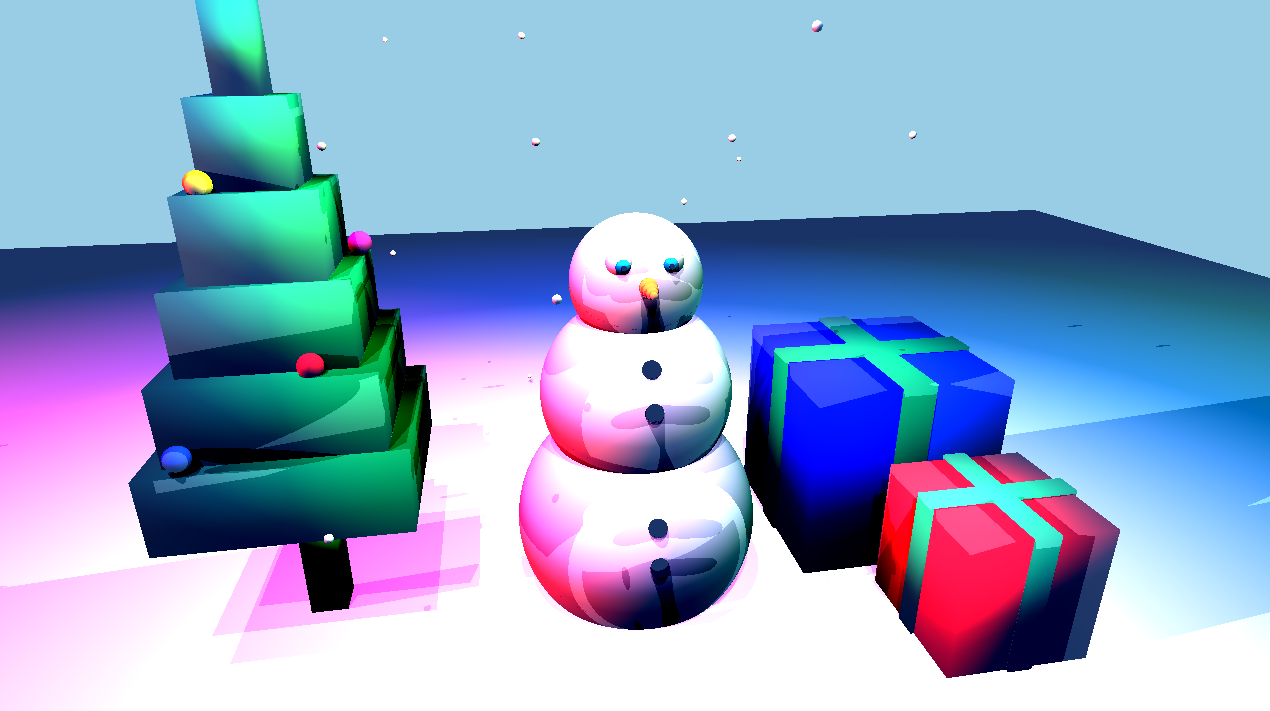
\includegraphics[width=0.4\linewidth]{ex2.png}
\hfill

\includegraphics[width=0.4\linewidth]{ex.png}
\hfill

\end{document}
